\documentclass[a4paper]{article}

\usepackage[utf8]{inputenc}
\usepackage[portuges]{babel}
\usepackage[T1]{fontenc}
\usepackage{graphicx}
\usepackage{a4wide}
\usepackage[pdftex]{hyperref}
\usepackage{float}
\usepackage{indentfirst}
\usepackage{subcaption}

\begin{document}

\title{Trabalho Prático\\ Sistemas Operativos\\Grupo 19}
\author{Catarina Machado (a81047) \and João Vilaça (a82339)}
\date{\today}

\begin{titlepage}

  %título
  \thispagestyle{empty}
  \begin{center}
  \begin{minipage}{0.75\linewidth}
      \centering
  %engenharia logo
      
\includegraphics[width=0.4\textwidth]{imgs/eng.jpeg}\par\vspace{1cm}
      \vspace{1.5cm}
  %titulos
      \href{https://www.uminho.pt/PT}{\scshape\LARGE Universidade do Minho} \par
      \vspace{1cm}
      \href{https://www.di.uminho.pt/}{\scshape\Large Departamento de Informática} \par
      \vspace{1.5cm}

  \maketitle
  \end{minipage}
  \end{center}

  \clearpage

 \end{titlepage}


\begin{abstract}
O presente relatório descreve o trabalho prático realizado no âmbito da disciplina de
\href{http://miei.di.uminho.pt/plano_estudos.html#sistemas_operativos}
{\emph {Sistemas Operativos} (SO)}, ao longo do segundo semestre,
do segundo ano, do \href{http://miei.di.uminho.pt}{Mestrado Integrado em Engenharia Informática}
da \href{https://www.uminho.pt}{Universidade do Minho}.

O objetivo do projeto foi construir um sistema para processamento de notebooks,
que misturam fragmentos de código, resultados da execução e documentação.
Neste contexto, um notebook é um ficheiro de texto que depois de processado é
modificado de modo a incorporar resultados da execução de código ou comandos nele embebidos.

Neste documento descrevemos sucintamente o sistema desenvolvido, as principais
funções utilizadas, bem como as decisões tomadas durante o
projeto.

\end{abstract}


\pagebreak

\tableofcontents

\pagebreak


\section{Introdução}
\label{sec:intro}

O presente relatório foi elaborado no âmbito da unidade curricular
\href{http://miei.di.uminho.pt/plano_estudos.html#sistemas_operativos}
{\emph {Sistemas Operativos} (SO)}, ao longo do segundo semestre,
do segundo ano, do \href{http://miei.di.uminho.pt}{Mestrado Integrado em Engenharia Informática}
da \href{https://www.uminho.pt}{Universidade do Minho}, e tem como objetivo
construir um sistema para processamento de notebooks que deverá ser um comando
onde dado um nome de ficheiro, interpreta-o, executa os comandos nele embebidos,
e acrescenta o resultado da execução dos comandos ao ficheiro.


\subsection{Descrição do Problema}
\label{sec:problema}

O projeto proposto implica desenvolver um programa onde dado um ficheiro, o programa
interpreta-o, tendo em consideração que as linhas começadas por ``\$'' são interpretadas como
comandos que serão executados, sendo o resultado produzido inserido imediatamente a seguir,
delimitado por $>>>$ e $<<<$. As linhas começadas por ''\$|'' executam comandos
que têm como \emph{stdin} o resultado do comando anterior (\textbf{Execução de programas}).\\

Para além disso, depois de processado pela primeira vez,
um notebook poderá ser editado pelo utilizador,
que poderá modificar os comandos a executar, e mais tarde processá-lo novamente.
O processador deverá então substituir os resultados do processamento anterior pelos novos resultados
(\textbf{Re-processamento de um notebook}).\\

Caso algum dos comandos não consiga ser executado,
não termine com sucesso, ou escreva algo para o $stderr$, o processamento deve ser abortado,
devendo o notebook ficar inalterado. O utilizador também deverá poder interromper
um processamento em curso, com ˆC, devendo o notebook permanecer inalterado
(\textbf{Deteção de erros e interrupção da execução}).\\

Como funcionalidade avançada, o programa deverá ter
\textbf{acesso a resultados de comandos anteriores arbitrários}, ou seja,
os comandos deverão poder ser generalizados para terem como $stdin$ o resultado
do n-ésimo comando anterior, com linhas começadas por \$n|, por exemplo \$4|
para se referir ao quarto comando anterior, sendo \$1| equivalente a \$|.
Esta funcionalidade deverá ser obtida evitando executar vários vezes o mesmo comando.\\

A última funcionalidade avançada é a \textbf{execução de conjuntos de comandos}.
Depois de ter a funcionar a execução de um comando
e respectivos argumentos, poderá ser acrescentado pipelines ou até execução concorrente.



\subsection{Conceção da Solução}
\label{sec:solucao}

Para resolvermos este problema foram cruciais três momentos. Numa primeira fase,
analisamos o problema e fizemos o ``parse'' do notebook, em segundo lugar passámos para
a elaboração da ``execution'' do mesmo e em último lugar fizemos o ``save'' dos resultados
do processamento no ficheiro. Elaborámos ainda os ``tests'', onde
fazemos vários testes ao programa de uma forma muito simples, rápida e eficiente.

O relatório está organizado da seguinte forma: a
Secção~\ref{sec:struct} apresenta a \textbf{estrutura de dados} utilizada, a
Secção~\ref{sec:parse} descreve o ficheiro parse e consequentemente a forma como
o \textbf{parse do notebook} é efetuada, a Secção~\ref{sec:execution} descreve a forma
como o \textbf{processamento do notebook} é feita no nosso programa
e a Secção~\ref{sec:save} refere-se à
forma como os \textbf{resultados do processamento são embebidos no ficheiro notebook}.
A Secção~\ref{sec:tests} refere-se à forma como implementamos o
mecanismo de \textbf{testes}
e, por último, a Secção~\ref{sec:mainandnps} descreve sucintamente
como o nosso programa se desenvolve a partir do momento em que é executado na linha
de comandos.



\section{Implementação}
\label{sec:implementacao}

Para a concretização do trabalho prático dividimos o nosso programa em
seis ficheiros, cada um com uma determinada tarefa,
o que contruibuiu para uma melhor organização,
gestão e manutenção do projeto.

Em seguida, explicamos a forma como resolvemos cada um dos problemas do
trabalho prático através das respetivas funções utilizadas:


\subsection{Struct}
\label{sec:struct}

A estrutura de dados utilizada foi a seguinte:

\begin{figure}[H]
\centering
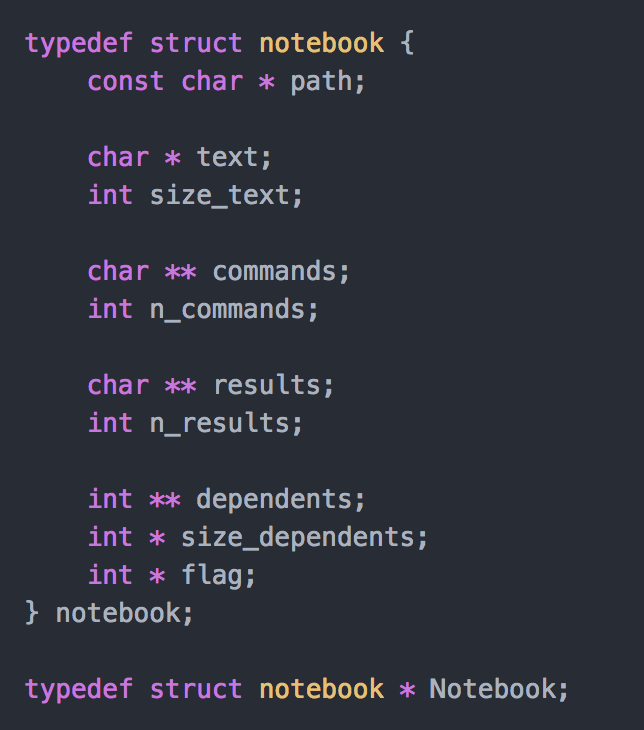
\includegraphics[scale=0.35]{imgs/struct.png}
\caption{Estrutura de Dados.}
\label{img:datastruct}
\end{figure}

A variável \textsf{path} armazena o caminho para o ficheiro notebook (passado
como parâmetro), a variável \textsf{text} guarda o texto contido no notebook
e a variável \textsf{size\_text} traduz o respetivo comprimento do texto.

A variável \textsf{commands} é um array de char * (strings), onde se encontram
os comandos das linhas começadas por ``\$'', ou seja, todos os comandos que terão
que ser executados. A variável \textsf{n\_commands} guarda o número total de comandos.

A variável \textsf{results} é também um array de char * (strings), que contém os
resultados da execução de cada um dos comandos. A variável \textsf{n\_results}
armazena o número de comandos que foram efetuados com sucesso, ou seja,
o número de resultados conseguidos.

A variável \textsf{dependents} é um array de arrays de inteiros,
onde para cada um dos comandos (cada comando corresponde a um inteiro,
que é o índice onde se encontra no array \textsf{commands}) está associado
um array com os índices dos comandos que dependem dele para serem executados.
Ou seja, cada comando possui um array com o identificador de todos os comandos
que dependem dele. Na variável \textsf{size\_dependents} estão armazenados,
para cada um dos comandos, o número de comandos que dependem dele.

Por último, a variável \textsf{flag}, um array de inteiros, que indica se
o comando pode ser executado (flag == 1) ou se não pode (flag == 0). Um comando
só pode ser executado se não depende de nenhum outro comando ou se o comando
que ele depende já foi executado.



\subsection{Parse}
\label{sec:parse}

Para efetuar o processamento do notebook é necessário inicialmente efetuar
o parse do mesmo. Para isso, temos uma função \textbf{get\_text} que vai lendo
o ficheiro de texto, 100 bytes de cada vez, e escrevendo-o na estrutura
de dados. A função devolve o número de caracteres lidos, que é também armazenado
na estrutura.

Depois disso, na função \textbf{parse}, vamos analisando o texto e preenchendo
a estrutura de dados, nomeadamente no que diz respeito aos comandos encontrados
(linhas que começam por ``\$''), às dependências entre os comandos e ao facto
de o comando se encontrar pronto ou não a ser executado.



\subsection{Execution}
\label{sec:execution}

Nesta fase, é percorrida a estrutura de dados e é executado cada comando
existente. Inicialmente são criados vários pipelines destinados a manter o
controlo do fluxo de dados resultantes da execução dos vários comandos, quer
seja para enviar e receber o seu resultado, verificar se algo foi escrito
para o $stderr$ ou até para enviar resultados de execuções anteriores a comandos
que estão neste momento a ser executados.\\
Na execução propriamente dita, o primeiro passo é verificar se o comando
recebe alguma argumento, ou seja, linhas começadas por ''\$'' ou ''\$|'' e,
em caso afirmativo, aceder ao resultado necessário e escrevê-lo para o pipeline
adequado e redirecionar o $stdin$ usado pelo execução para esse pipeline.
Neste momento, é apenas necessário processar o comando que será executado,
nomeadamente verificar se existem múltiplos pipelines para se encadear os seus
resultados e dividir este comando em vários argumentos para que a execução
seja feita recorrendo ao uso da função
$int execvp(const char *file, char *const argv[]);$.
Finalmente é apenas necessário ler o resultado final do $stdout$ e armazená-lo
na estrutura de dados.


\subsection{Save}
\label{sec:save}

Nesta última fase do programa, onde já está assegurado que todos os comandos
foram executados com sucesso, o ficheiro notebook é aberto e reescrito.
Toda a informação necessária para tal está armazenada na estrutura de dados, e
tanto os comentários/documentação, como os comandos e os respetivos
resultados de execução
(delimitados por $>>>$ e $<<<$) são escritos no ficheiro, eliminando o
texto inicialmente escrito.



\subsection{Tests}
\label{sec:tests}

Este programa tem implementado um mecanismo de testes automáticos do sofware.
Este testes podem ser efetuados executando o programa com o argumento $test$.
Eles estão implementados de maneira relativamente simples. Existe uma diretoria
\emph{test\_dir} sobre a qual serão executados todos os comandos para os
resultados serem constantes, existe também uma outra diretoria que contém os
ficheiros de \emph{input} que serão usados na execução do programa, e ainda, a
\emph{output}, que contém os resultados esperados, os quais serão comparados
com produto final da execução do programa.
Cria-se uma cópia do ficheiro de $input$, sobre a qual é executado
verdadeiramente o programa, de modo a não alterar o ficheiro original, no fim
estes são comparados através de um $diff$ seguido de um $wc$ para verificar se
existem diferenças entre o obtido e o resultado esperado, se não as houver o
resultado está certo, se existirem diferenças o teste falha e o ficheiro cópia
é mantido para se poder analizar o resultado.
Neste momento existem 5 testes, em que cada um deles verifica uma ou mais
funcionalidades do projeto. O $exec$ que verifica a correta execução do
programa, comando simples $\$ ls$, comandos com pipelines $\$ls | wc$ e acesso
a resultados de comandos executados anteriormente
$\$3| sort --reverse | head -1$.

\begin{figure}[H]
\centering
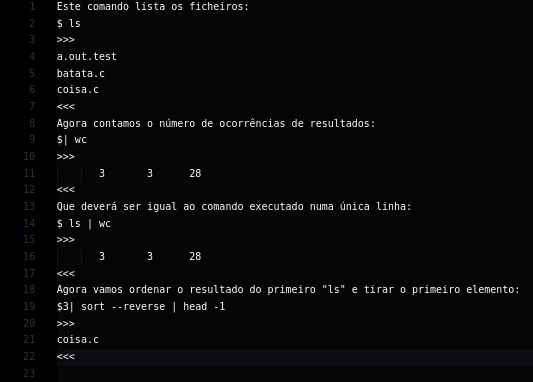
\includegraphics[scale=0.35]{imgs/exec.png}
\caption{Exec}
\label{img:Exec}
\end{figure}

O $stderr$ e o $erros$ que verificam se a
execução é cancelada e se o ficheiro permanece inalterado caso algo seja
escrito para o stderr ou caso a execução de um comando falhe respetivamente.

\begin{figure}[H]
\centering
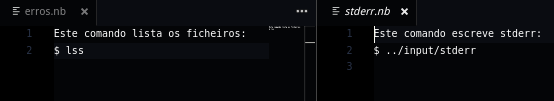
\includegraphics[scale=0.35]{imgs/erros.png}
\caption{Erros e escrita para stderr}
\label{img:Erros}
\end{figure}

O $empty$ e $text$ que verificam que se para um ficheiro vazio ou só com texto
também eles permanecem inalterados.

\begin{figure}[H]
\centering
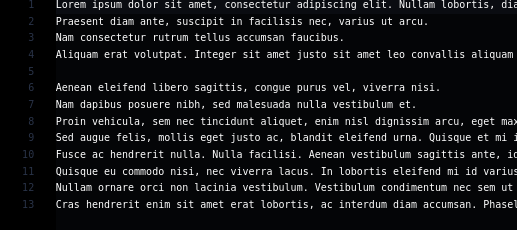
\includegraphics[scale=0.35]{imgs/text.png}
\caption{Text}
\label{img:Text}
\end{figure}


Todos os testes foram efetuados com sucesso.

\begin{figure}[H]
\centering
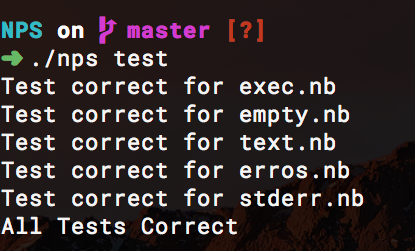
\includegraphics[scale=0.35]{imgs/results.png}
\caption{Resultados}
\label{img:Resultados}
\end{figure}


\subsection{Main \& NPS}
\label{sec:mainandnps}

O ficheiro \textbf{main} verifica se o número de argumentos do programa é valido
(tem que ser obrigatoriamente um, o $path$), e em caso afirmativo são executados:
os testes automáticos, se o path passado for \textbf{test}, ou é executada a função
\textbf{nps}, que processa o ficheiro no path passado como argumento.

A função \textbf{nps} aloca o espaço necessário para armazenar a estrutura de dados,
executa as funções de \textbf{parse} e de \textbf{execute} e no caso
da execução ter sido concluída com sucesso, os resultados
são escritos no ficheiro notebook com recurso à função \textbf{save}. Por fim,
é liberado todo o espaço alocado.



\section{Conclusões}
\label{sec:conclusao}

Face ao problema apresentado e analisando criticamente a solução proposta
concluímos que cumprimos as tarefas, conseguindo atingir os objetivos definidos.
De facto, foram implementadas todas as funcionalidades apresentadas, quer
básicas quer avançadas.
Deste modo, foi então construído um sistema de processamento de notebooks
perfeitamente funcional, com testes automáticos para todas as suas
funcionalidades implementadas que provam o correto funcionamento do mesmo.


\end{document}
